\section{Rilevamento movimento ambientale}
All'interno dell'applicazione l'apparato visivo del dispositivo viene utilizzato per eseguire \textit{motion detection}.\\
Qualora tale impostazione venga abilitata è necessario esaminare le immagini catturate dal dispositivo per determinare se v'è stato del movimento all'interno del raggio visivo: ad intervalli regolari le foto scattate dalla fotocamera vengono esaminate e confrontate per determinare il movimento. Qualora l'algoritmo di \textit{motion detection} ritenga di aver determinato del movimento, tale stato viene notificato e si tenterà di conseguenza di spedire le immagini catturate al server predisposto e di notificare l'utente di una possibile intrusione.\\

\noindent Le immagini catturate sono utilizzate per due ruoli fondamentali:
\begin{enumerate}
  \item Sono i dati di input per l'algoritmo di \textit{motion detection}. In questo caso il ruolo che svolgono è statistico in quanto l'algoritmo utilizzato non è sofisticato e specifico per il riconoscimento di movimento umano
  \item Sono informazioni mnemoniche spedite al server incaricato al loro stoccaggio. In questo caso il ruolo che svolgono è semantico in quanto utilizzate dall'utente finale per riconoscere o meno un'intrusione
\end{enumerate}
\noindent Le immagini vengono inoltre utilizzate dall'applicazione per fornire all'utente un riscontro visivo di quel che l'applicazione rileva come movimento. All'interno dell'applicazione è stata appositamente creata una schermata che riassume lo stato della \textit{motion detection} come illustrato in figura \ref{fig:motionDetection}.
\begin{figure}[!ht]
\begin{center}
\begin{minipage}[r]{.5\textwidth}
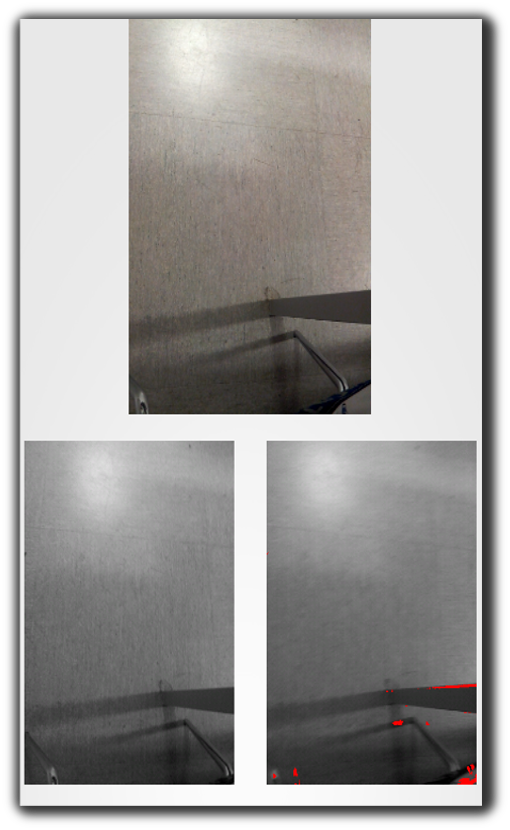
\includegraphics[scale=.3]{./../wireless/resources/camera.png}
\end{minipage}
\begin{minipage}[l]{.4\textwidth}
\caption{Schermata offerta dall'applicazione per il rilevamento del movimento ambientale.\\ L'immagine in alto corrisponde allo stream di immagini catturate dalla camera.\\ Le immagini in basso rappresentano gli ultimi due frame elaborati: l'immagine a sinistra rappresenta il penultimo frame catturato mentre l'immagine a destra rappresenta l'ultimo frame catturato in cui si evidenziano in rosso le porzioni d'immagine in cui è stato rilevato del movimento.}
\label{fig:motionDetection}
\end{minipage}
\end{center}
\end{figure}


\subsection{Motion detection}
L'algoritmo di \textit{motion detection} determina il movimento confrontando due immagini in scala di grigi. Le immagini vengono acquisite ad intervalli regolari di 1 secondo.\\
Qualora la differenza tra queste due immagini sia superiore ad una certa soglia si identifica la presenza di movimento. I valori di soglia definiti hanno influenza su due componenti all'interno dell'algoritmo:
\begin{enumerate}
  \item Poiché le immagini sono una collezione di pixel, il loro confronto avviene a tale livello. Risulta molto improbabile, anche in assenza di movimento, che due immagini consecutive abbiano i pixel corrispondenti identici: ad esempio una variazione di luminosità all'interno della stanza può essere causata dal passaggio di una nuvola, e tale variazione di luminosità è quello che si considera per determinare il movimento. \`E quindi necessario determinare un valore di soglia entro il quale due pixel, anche se non identici, vengono considerati non sostanzialmente differenti e non contribuiscono quindi a differenziare le immagini considerate.\\
  Questo valore di soglia viene applicato al confronto pixel a pixel.
  \item La differenza tra due immagini viene eseguita pixel per pixel. Risulta molto improbabile, anche in assenza di movimento, che due immagini consecutive abbiano tutti i pixel corrispondenti uguali: ad esempio uno spiffero d'aria può far muovere delle tende o dei vestiti. \`E quindi necessario determinare un valore di soglia che permetta di distinguere quando la differenza tra le immagini considerate sia trascurabile.\\
  Questo valore di soglia viene applicato sul conteggio di pixel che son variati da un'immagine alla successiva.
\end{enumerate}
L'utente può quindi specificare la sensibilità per il rilevamento del movimento all'avvio dell'applicazione. I valori disponibili e i relativi parametri sono:
\begin{itemize}
  \item \texttt{LOW}: una sensibilità bassa. Permette una variazione di luminosità del 24\% per pixel (ossia la differenza tra due pixel deve essere compresa all'intervallo $[0,60]$) e determina il movimento qualora il 6.5\% dell'immagine sia cambiata (ossia qualora vengano determinati più di $20000$ pixel differenti).
  \item \texttt{MEDIUM}: una sensibilità media. Permette una variazione di luminosità del 20\% per pixel (ossia la differenza tra due pixel deve essere compresa all'intervallo $[0,50]$) e determina il movimento qualora il 3.2\% dell'immagine sia cambiata (ossia qualora vengano determinati più di $10000$ pixel differenti).
  \item \texttt{HIGH}: una sensibilità alta. Permette una variazione di luminosità del 16\% per pixel (ossia la differenza tra due pixel deve essere compresa all'intervallo $[0,40]$) e determina il movimento qualora il 2.9\% dell'immagine sia cambiata (ossia qualora vengano determinati più di $9000$ pixel differenti).
\end{itemize}

\subsection{Stoccaggio immagini}
Qualora l'algoritmo di \textit{motion detection} ritenga di aver rilevato del movimento viene attivato il meccanismo incaricato di notificare l'avvenimento. Tale notifica varia a seconda delle impostazioni scelte dall'utente e dall'ambiente in cui si trova il dispositivo. Qualora l'opzione di notificare il server sia stata abilitata e l'ambiente lo permetta (sia presente una rete WiFi o vi sia collegamento 3G) le immagini catturate vengono spedite al server in attesa di essere consultate dall'utente.\\
A seconda della connettività il numero delle immagini inviate variano:
\begin{itemize}
  \item Accesso WiFi: vengono spedite 10 immagini
  \item Accesso 3G: vengono spedite 5 immagini
\end{itemize}

\subsection{Formati immagine utilizzati}
L'acquisizione ed il formato delle immagini è un punto fondamentale per questa parte di applicazione: poiché si tenta di acquisire immagini ad intervalli di 1 secondo è importante che l'elaborazione di tali immagini non diventi un collo di bottiglia.\\

Per ridurre il più possibile computazioni non necessarie o onerose è fondamentale utilizzare un formato immagine adatto agli scopi, a patto che tale conversione non diventi un carico ingente di computazione.\\

\subsubsection{YUV NV21}
Si è quindi deciso di acquisire le immagini in formato NV21.\\
Tale formato si basa sullo spazio di colore YCbCr (anche se normalmente il formato viene identificato come YUV NV21\footnote{ Lo spazio colore YUV viene storicamente utilizzato per denotare codifiche di colori per segnali analogici, mentre YCbCr viene utilizzato per segnali digitali.}) con campionatura 4:2:0 (ossia entrambe le componenti di crominanza vengono sottocampionate di un fattore due sia in verticale che in orizzontale come evidenziato dalla figura \ref{YUVsampling}).\\
\begin{figure}[!ht]
\begin{center}
\YUVsampling
\end{center}
\caption{Esempio di campionatura in spazio colore YCbCr $4:2:0$ di un'immagine di dimensioni $6×4$ pixel.}
\label{YUVsampling}
\end{figure}

\noindent In particolare il formato NV21 definisce come le informazioni di luma e crominanza vengono organizzate. Questo formato è un formato semiplanare in quanto le informazioni di luma sono memorizzate separatamente dalle informazioni di crominanza: 
\begin{itemize}
  \item Viene definito un piano per la componente Y. La dimensione di questo piano è esattamente la dimensione dell'immagine in quanto questa componente non viene sottocampionata, ossia è presente una componente per ogni pixel dell'immagine
  \item Viene definito un piano condiviso per le componenti di crominanza U e V. La dimensione di questo piano è la metà del piano relativo alla componente Y in quanto le componenti di crominanza vengono sottocampionate di un fattore due (e quindi ogni componente di crominanza occupa un quarto della dimensione di luminanza).\\
  I valori campionati di U e V vengono memorizzati interlacciati (in quanto sono compresenti sullo stesso piano) e a partire dalla componente V come evidenziato dalla figura \ref{YUVplanes}.\\
\end{itemize}
\begin{figure}[!ht]
\begin{center}
\subfigure[Piano per i campioni luminanza]{\YUVplanesLuma}~
\subfigure[Piano per i campioni crominanza]{\YUVpanesCroma}
\end{center}
\caption{Suddivisione dell'informazione visiva: piano dedicato all'informazione relativa esclusivamente alla luminanza e piano condiviso per l'informazione sulla crominanza blu e rossa.}
\label{YUVplanes}
\end{figure}

\noindent Quello che si ottiene a livello di applicazione attraverso l'acquisizione da fotocamera è in realtà uno stream di byte unico in cui i piani (di luma e crominanza) vengono concatenati come mostrato in figura \ref{YUVbytestream}.
\begin{figure}[!ht]
\begin{center}
\makebox[\linewidth]{\YUVbytestream}
\end{center}
\caption{Serializzazione dei valori nel bytestream.}
\label{YUVbytestream}
\end{figure}


L'utilizzo del formato NV21 comporta diversi vantaggi:
\begin{itemize}
  \item \`E il formato standard di acquisizione dei dispositivi Android: non è quindi necessario interrogare ogni volta il dispositivo per determinare i possibili formati di acquisizione. Avendo sempre a disposizione un unico formato è stato possibile definire una sola routine in grado di convertire immagini da questo formato a scala di grigi (formato utilizzato per il \textit{motion detection})
  \item Poiché tale formato è standard nei vari dispositivi c'è la garanzia che le prestazioni per l'acquisizione dell'immagine in tale formato siano migliori delle prestazioni ottenute dovendo operare una conversione ad hoc a livello applicazione
  \item Attraverso questo formato risulta immediato ottenere un'immagine in scala di grigi in quanto la componente luma è esplicitata: non son quindi necessarie conversioni più onerose come potrebbe essere la conversione da RGB a scala di grigi
  \item La struttura di questo formato è adatta ad operare su dispositivi mobili: la sua struttura interna riduce considerevolmente gli accessi in memoria in quanto le varie componenti sono salvate in locazioni di memoria abbastanza contigue.\\
  L'hardware incaricato all'acquisizione risulta inefficiente se per ogni pixel è necessario accedere in locazioni differenti di memoria (un accesso per ogni piano in cui devono venir memorizzate le varie componenti come per esempio RGB o YUV I444): la situazione ottimale per l'acquisizione si raggiungerebbe utilizzando un formato pacchettizzato, ma un formato semi-planare è comunque meglio di un formato planare.\\
  Per quanto riguarda l'elaborazione, il formato NV21 risulta invece ottimale: l'informazione principalmente utilizzata per l'elaborazione è quella relativa alla componente luma che è memorizzata in maniera contigua.
\end{itemize}

Per ridurre ulteriormente il carico di lavoro, poiché non interessa un'alta definizione per le immagini, viene impostata la fotocamera ad acquisire le immagini a risoluzione minore possibile (la scelta di default è $640×480$):
\begin{itemize}
  \item Si evita un consumo di memoria eccessiva in quanto tali immagini devono venire successivamente salvate
  \item Poiché il tempo di creazione di un oggetto è limitato inferiormente dalla quantità di memoria che necessita, avere un'immagine di dimensioni minori permette una sua creazione celermente
  \item Si evita di dover utilizzare procedure di scaling definite dall'applicazione (che sarebbero meno efficienti delle procedure definite dall'hardware della fotocamera o dei suoi driver)
\end{itemize}

\subsubsection{RGB565}

Nonostante l'informazione contenuta all'interno del formato NV21 sia sufficiente per applicare l'algoritmo di \textit{motion detection}, si è preferito estrarre esplicitamente l'informazione relativa alla luminanza e trattarla come informazione in scala di grigi. Questo procedimento viene eseguito principalmente per due motivi:
\begin{enumerate}
  \item Dopo l'elaborazione per \textit{motion detection} siamo interessati a costruire un'immagine in scala di grigi. Risulta quindi utile avere a disposizione direttamente tale informazione. L'immagine in scala di grigi viene utilizzata per fornire all'utente il display delle differenze notate tra due immagini consecutive. Avendo a disposizione un'immagine in scala di grigi risulta immediato un meccanismo per evidenziare le zone dell'immagine in cui è stato determinato il movimento: è sufficiente colorare tali zone con un colore acceso (per esempio si utilizza il rosso) di modo che vi sia sufficiente contrasto con l'immagine di sfondo (che è appunto in scala di grigi)
  \item Java non offre operatori binari in grado di operare sui byte. Per evitare di affidarsi a conversioni implicite incontrollate si è preferito operare consapevolmente tali operazioni e assicurarsi di non causare errori
\end{enumerate}

La conversione in scala di grigi passa attraverso due fasi:
\begin{enumerate}
  \item Ottenere l'esatta informazione sulla tonalità di grigio
  \item Costruire un'immagine in scala di grigi
\end{enumerate}

Attraverso la prima fase si ottiene una sequenza di \texttt{imageHeight×imageWidth} valori che corrispondono alla tonalità di grigio dei pixel dell'immagine. Su questa informazione viene applicato l'algoritmo di motion detection.\\
Considerando le relazioni che intercorrono tra lo spazio di colori YCbCr e RGB
\[
\left[\begin{array}{c}R\\G\\B\end{array}\right] = \left[
\begin{array}{ccc}1.164&0.000&1.793\\1.164&-0.213&-0.533\\1.164&2.112&0.000\end{array}
\right]\cdot \left[\begin{array}{c}(Y-16)\\(Cb-128)\\(Cr-128)\end{array}\right]
\]
la conversione tra l'informazione Y a informazione di grigio risulta pressoché immediata: è sufficiente operare una singola sottrazione.\\
Da notare che la conversione a scala di grigi viene effettuata sfruttando la struttura del formato NV21 in quanto l'informazione luma viene acceduta sequenzialmente (minimizzando in questo modo gli accessi in memoria) per produrre ordinatamente i pixel dell'immagine in scala di grigi.\\

La seconda fase consiste nel creare un'immagine a partire dall'informazione di grigio appena estratta.\\
Per poter operare la visualizzazione di un immagine all'interno di un dispositivo Android è necessario utilizzare l'apposita classe \texttt{Bitmap}. Sfortunatamente questa classe non supporta il formato di immagini in scala di grigi ma formati RGB o ARGB: non è possibile costruire quindi una \texttt{Bitmap} con un solo canale (corrispondente alla sfumatura di grigio) ma è necessario costruire una \texttt{Bitmap} con almeno 3 canali. Si è quindi reso necessario trasformare l'informazione sulla tonalità di grigio in informazione RGB (ossia replicare la luminosità in ogni canale RGB di modo da ottenere la tonalità di grigio voluta).
\[\text{GRAY}(x) \to \text{RGB}(x, x, x) \qquad x \in [0 \ldots 255] \]
L'utilizzo di una \texttt{Bitmap} a tre canali ha avuto comunque il vantaggio di poter manipolare l'immagine stessa per evidenziare le zone determinate da \textit{motion detection}. Avendo a disposizione tre canali è possibile cambiare l'informazione di un pixel per fargli assumere un qualsiasi colore, e non solo una sfumatura di grigio come sarebbe accaduto se si fosse utilizzata un'immagine ad un solo canale. Questa possibilità risulta molto utile per evidenziare le porzioni dell'immagine sulle quali l'algoritmo di \textit{motion detection} ha determinato del movimento.\\
I formati disponibili per la \texttt{Bitmap} sono:
\begin{itemize}
  \item ALPHA8: immagine che memorizza il solo canale di trasparenza
  \item ARGB4444: immagine che utilizza 2 byte per memorizzare un pixel, in cui l'informazione viene ripartita equamente tra le quattro componenti (ossia si hanno 4 bit o 16 valori per ogni componente)
  \item ARGB8888: immagine che per ognuna delle quattro componenti utilizza un byte
  \item RGB565: immagine che memorizza solo le componenti colore ma non la componente di trasparenza ed utilizza due byte per ogni pixel. L'informazione viene memorizzata non equamente in quanto vengono assegnati 5 bit per i canali rosso e blu e 6 bit per il canale verde
\end{itemize}
Si è deciso di utilizzare il formato RGB565 in quanto:
\begin{enumerate}
  \item Il formato ALPHA8 risulta inutile ai nostri scopi in quanto la trasparenza è l'unica informazione che non viene utilizzata
  \item Il formato ARGB444 risulta in una qualità estremamente scadente. Inoltre, poiché non interessa la trasparenza, la presenza dell'\textit{alpha channel} impiega inutilmente dei bit che potrebbero essere utilizzati per memorizzare altre informazioni
  \item Il formato ARGB888, nonostante sia il più completo, si sarebbe tradotto in un utilizzo di memoria eccessivo per l'uso che si fa dell'immagine. La presenza dell'\textit{alpha channel} risulta inutile (in quanto non si utilizza trasparenza) e non è necessaria un'alta qualità dell'immagine
  \item Il formato RGB565 si traduce in un'occupazione di memoria moderata con una più che discreta qualità dell'immagine. La mancanza del canale di trasparenza si traduce con l'assenza di spreco di memoria. Nonostante venga consigliato di utilizzare questo formato immagine in presenza di qualche filtro di dithering per evitare che lo sbilanciamento d'informazione verso il canale verde (6 bit contro i 5 bit dei canali rosso e blu) si traduca con una sfumatura verdognola dell'immagine, nella nostra applicazione non viene applicato nessun filtro in quanto:
  \begin{itemize}
    \item Applicare un filtro consumerebbe preziose risorse (energia e tempo)
    \item Lavorando con un'immagine in scala di grigi più un colore vivace (per evidenziare le zone di movimento) non interessa minimamente una possibile sfumatura verdognola dell'immagine
  \end{itemize}
\end{enumerate}
Considerando quindi che:
\begin{itemize}
  \item La qualità del colore dell'immagine di cui si fa il display è irrilevante in quanto l'immagine visualizzata è sostanzialmente un'immagine in scala di grigi
  \item L'immagine visualizzata cambia con una frequenza piuttosto elevata (1 volta al secondo circa) e non è quindi necessario che abbia una definizione elevata
  \item L'utilizzo di un formato che permetta di risparmiare memoria permette una manipolazione più veloce dell'immagine stessa
\end{itemize}
è parso che il formato RGB565 fosse il più adatto ai nostri scopi.

\subsubsection{JPEG}
Viene utilizzato il formato JPEG per salvare le immagini.\\
Qualora si rilevasse del movimento e fosse disponibile una connessione di rete sarebbe necessario inviare le immagini scattate al server dedicato al raccoglimento di tali informazioni. Il formato JPEG è il formato più idoneo a questo scopo in quanto:
\begin{itemize}
  \item Non è necessario modificare l'immagine.\\
  Le immagini visualizzate su dispositivo potevano richiedere una manipolazione (per evidenziare le zone di movimento): era quindi utile utilizzare un formato che permettesse una loro modifica in maniera istantanea senza dover utilizzare algoritmi di compressione e decompressione per effettuare tali cambiamenti. Una bitmap RGB era la soluzione ideale.\\
  Le immagini spedite al server non hanno necessità di essere modificate e non è quindi necessario utilizzare formati che facilitino tale operazione. Utilizzare il formato JPEG non causa quindi nessun problema
  \item \`E fortemente desiderabile che l'immagine occupi meno spazio possibile:
  \begin{itemize}
    \item L'immagine deve essere salvata sulla memoria del dispositivo in quanto, in caso di necessità, deve essere spedita al server incaricato alla raccolta delle informazioni. Considerando la limitata capacità di memoria dei dispositivi è bene risparmiare più spazio possibile
    \item Qualora l'immagine debba venir spedita sulla rete è estremamente desiderabile che l'informazione da inviare sia minima. Avere immagini di piccole dimensioni fa in modo che il processo di upload sia il più veloce possibile e permette di non sovraccaricare la banda disponibile (soprattutto qualora si sia connessi attraverso 3G)
  \end{itemize}
  Il formato JPEG è rinomato per la sua capacità di compressione ed è quindi ideale per ottenere immagini di dimensioni contenute
\end{itemize}

